\section{Another primal-dual algorithm for Joint Replenishment Problem}

\subsection{Preliminaries}
Joint replenishment problem is a well-studied problem in operations research community. Here we consider the deterministic version. Let's formally define the problem. There are $N$ item types numbered $1,2,\ldots,N$. And our whole planning horizon is discrete time $1,2,\ldots, T$. There are a set of demands and each demand is a pair $(i,t)$ where $i$ is the item type of the demand and $t$ is the time when this demand arrives. To satisfy demands, we place orders during our planning horizon. If we make a order consisting of items $S$ at time $s$, it will costs $K_0+\sum_{i\in S} K_i$, and can be used to satisfy demand $(i,t)$ arrives no later than $s$ and $i \in S$, notice here the cost of order doesn't depends on demands quantity of each item type satisfied. To balance the ordering cost, we also have delay cost. If a demand $(i,t)$ is satisfied at some later time $s$, then it incurs delay cost $w_{its}$. The only assumption we have about $w_{its}$ is that it's nondecreasing with respect to $s$. The objective is to satisfy all demands with minimum sum of ordering cost and delay cost.

The main result of this paper is the following
\begin{theorem}
There exists a primal dual 2-approximation algorithm without pruning stage for Joint Replenishment Problem.
\end{theorem}

\subsection{LP formulation}
We start by formulate the primal and dual LP of this problem, let $C(S) = K_0 + \sum_i K_i$ be the ordering cost of set of items $S$ and $\Delta_{its} = w_{it,s+1} - w_{its}$ be the incremental delaying cost, then the primal LP is
\begin{align}
	\min \quad & \sum C(S) x(S,t) + \sum \Delta_{its}z(i,t,s) \\
	s.t \quad& \sum_{S \ni i} \sum_{r=t}^s x(S,r) + z(i,t,s) \ge 1
\end{align}
Here we use $x(S,t)$ to denote whether we put a order of set $S$ at time $t$, $z(i,t,s)$ indicate whether demand $(i,t)$ need to wait from time $s$ to $s+1$. The constraint says that if there is no ordering containing $i$ from time $t$ to $s$(inclusive), then demand $(i,t)$ need to incur the incremental delay cost $\Delta_{its}$.

The dual provides a different view of this problem in term of budget
\begin{align}
	\max \quad & \sum y(i,t,s) \\
	s.t \quad & y(i,t,s) \le \Delta_{its} \\
	& \sum_{(i,t) | t \le s} \sum_{r\ge s} y(i,t,r) \le C(S) \label{dualorder}
\end{align}
We can view $y(i,t,s)$ as the budge of demand $(i,t)$ towards paying the incremental cost $\Delta_{its}$. Imagine that we have a potential ordering $S$ at time $s$, then the second constraint says that for all the demands which can be served by this ordering, after paying the delaying cost, the remaining budget should be at most the ordering cost of $S$.

\subsection{Algorithm}
In this section, we describe our algorithm. This is a primal-dual algorithm different than the previous one \cite{levi2006primal} and this is a simplification of online primal-dual algorithm of \cite{buchbinder2008online}. Although the dual ascent phase is exact the same as in \cite{levi2006primal}, we construct different primal solution here. In addition, there is no pruning phase in the end.

At the beginning of the algorithm, we set all $y(i,t,s)$ to be zero. The progress of this algorithm is captured by the notion of time $\tau$, which starts at zero and increases with unit speed. The state of a demand can be either active or inactive. Active demands are those demands which haven't been satisfied and arrived before $\tau$. Inactive ones are those served already. At the same time when we increase time $\tau$, we also increase dual variables $y(i,t,s)$ for active demands $(i,t)$. We start to increase $y(i,t,s)$ from 0 when $\tau$ reaches $s$ and freeze $y(i,t,s)=\Delta_{its}$ when $\tau$ reaches $s+1$.

During the algorithm, we keep track of the time $\hat s$ of last order placed. There are two kinds of events. Event I is when there is some order $S$ at $s > \hat s$ just becomes payed for, i.e. the second constraint (\ref{dualorder}) becomes tight for some $S$ and $s > \hat s$, then we place order $S$ at current time $\tau$. Event II is when there is some $(i,s)$ such that $\sum_{(i,t): t\le s} \sum_{r\ge s} y(i,t,r) \ge K_i$ for $s \le \hat s$. In this case, we augment order at $\hat s$ by adding $i$ to the existing order. In either event, we serve all demands reachable from newly placed order and mark them inactive. The algorithm keeps increasing time $\tau$ until all demands are satisfied.

You may doubt whether these are all the events can ever happen for the dual ascent algorithm without violating dual constrains. Notice that whenever a constraint in (\ref{dualorder}) becomes tight for $(S,s)$, it corresponds to Event I if $s > \hat s$. If $s \le \hat s$, there must be some $i \in S$ such that $\sum_{(i,t): t\le s} \sum_{r\ge s} y(i,t,r) \ge K_i$ before $(S,s)$ becomes tight because demands only start to contribute to joint ordering cost after they paid for item ordering cost.

\begin{algorithm}
\begin{algorithmic}
\State During the algorithm let $\hat s$ be the time of last order
\While{there exists demand not served}
\State Increase $\tau$ and $y(i,t,s)$ for active demands $(i,t)$ until
\If{There exists some $(S,s)$ such that (\ref{dualorder}) becomes tight for $s >\hat s$}
\State Place order $S$ at current time $\tau$
\ElsIf{There exists some $(i,s)$ such that $\sum_{(i,t): t\le s} \sum_{r\ge s} y(i,t,r) \ge K_i$}
\State Augment order at $\hat s$ by adding $i$ to existing order
\EndIf
\EndWhile
\end{algorithmic}
\caption{Primal dual algorithm}
\end{algorithm}

\subsection{Analysis}
In this section, we prove the above algorithm is $2$-approximation. As in other primal-dual algorithm, we will bound the cost of constructed primal against dual solution. More specifically, we will devise a charging scheme such that each nonzero dual $y(i,t,s)$ is charged at most twice.

First let's introduce some notations. For an inactive demand $(i,t)$, let $\alpha(i,t)$ be the time of order we use to serve $(i,t)$ and let $\beta(i,t)$ is the time when we mark $(i,t)$ inactive. Notice here that $t \le \alpha(i,t) \le \beta(,t)$. For active demand $(i,t)$, $\beta(i,t)$ is defined to be current time $\tau$ and $\alpha(i,t)$ is defined to be $t$. Notice $y(i,t,s)$ is nonzero only if $s \in [t, \beta(i,t)]$. We can define the notation of a demand $(i,t)$ contributes to a order as following. In Event I, we say $(i,t)$ contributes to order $(S,s)$ if $i \in s$ and $s \in [t, \beta(i,t)]$. In Event II, we say $(i,t)$ contributes to order $(i,s)$ if $s \in [t, \beta(i,t)]$.

Now we can describe our charging scheme. We need to charge both delay costs for newly served demands and order cost. We know that $y(i,t,s)$ represents budget of demand $(i,t)$ for interval $[s,s+1]$, in the following, we use $Y(i,t,a,b) = \sum_{r = a}^{b-1} y(i,t,s)$ to denote the total budge of $(i,t)$ for interval $[a,b]$.

For Event I, we charge each active contributing demand $(i,t)$ amount $Y(i,t,t,\tau)$ for delay cost. We charge each contributing demand $(i,t)$ amount $Y(i,t,\alpha(i,t),\beta(i,t)$ for order cost. We're going to prove that we actually charged more than need. In total, we covered our order cost and delay cost for Event I case.

For Event II, we only need to collect $K_i$ for order cost in total. We charge each contributing demand $(i,t)$ amount$Y(i,t,\alpha(i,t),\beta(i,t)$. Again, we'll prove we charged enough. Also, for each active contributing demand $(i,t)$, we charge it $Y(i,t,t,\hat s)$ for delay cost.

We'll start by proving some easy facts.

\begin{figure}
\centering
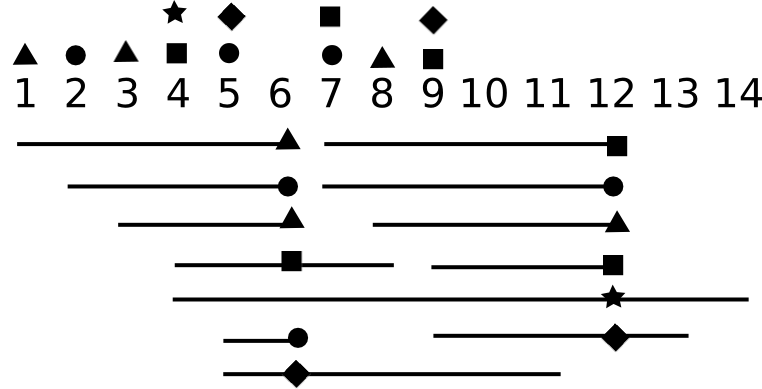
\includegraphics[width=.7\linewidth]{other/jrp}
\caption{Example of running algorithm. Here the delay cost is unit cost, $K = 5$, fix ordering cost: triangle 2, circle 2, rectangle 4, star 10, diamond 6}
\end{figure}

\begin{lemma}
For inactive demand $(i,t)$ such that $\alpha(i,t)$ is strictly smaller than $\beta(i,t)$, there is no order within $(\alpha(i,t), \beta(i,t)]$. \label{lem:overlap}
\end{lemma}
\begin{proof}
The only case when $\alpha(i,t) < \beta(i,t)$ happens is when $(i,t)$ is included in an augmented order. In that case, remember that we put order at the time of last order. Suppose there is order within $(\alpha(i,t), \beta(i,t)]$, it must be already there when the Event II happens because we only place totally new order at current time. This contradict our choice to augment order at latest order available.
\end{proof}

For the sake of notation, let's define $\hat s_i$ to be the time of last order including $i$.

\begin{lemma}
In Event I for tight set $(S,s)$, the tight time $s$ is strictly larger than $\hat s_i$ for any $i\in S$. In Event II for $(i,s)$, $s$ is strictly larger than $\hat s_i$. \label{lem:larger}
\end{lemma}
\begin{proof}
In Event I, $s > \hat s$ so $s > \hat s_i$ trivially. In Event II, there is at least one active demand $(i,t)$ of type $i$ contributing. This implies $s \ge t$, we also know that since $(i,t)$ is active $t > \hat s_i$ because otherwise it's already served and must be inactive. Thus, $s > \hat s_i$.
\end{proof}

\begin{lemma}
For inactive demand $(i,t)$, it can be charged in the future only if $\alpha(i,t) = \hat s_i$. \label{lem:charge}
\end{lemma}
\begin{proof}
Suppose $(i,t)$ is served by order earlier than $\hat s_i$. Suppose in the future we place some order for tight set $(S,s)$. If item $i$ is involved, then because there is at least one active contributing demand of type $i$, we know $s > \hat s_i$. While for $(i,t)$, by Lemma \ref{lem:overlap}, there is no order within $(\alpha(i,t), \beta(i,t)]$, it must be that $\hat s_i > \beta(i,t)$ which implies $(i,t)$ cannot contributes to $(S,s)$.
\end{proof}

\begin{lemma}
Our charging scheme charged enough to pay for order cost.
\end{lemma}
\begin{proof}
For each contributing order $(i,t)$, we charged $Y(i,t,\alpha(i,t),\beta(i,t))$ for order cost but we actually need to charge$Y(i,t,s,\beta(i,t))$. So we just need to prove $\alpha(i,t) \le s$. For active order, since $\alpha(i,t) = t$, it's trivial. For inactive order, by Lemma \ref{lem:larger}, we know $s > \hat s_i \ge \alpha(i,t)$.
\end{proof}

Now we can prove our main theorem

\begin{theorem}
There exists a primal dual 2-approximation algorithm without pruning stage for Joint Replenishment Problem.
\end{theorem}
\begin{proof}
We prove this by showing an invariant of the algorithm. We want to show that at any time, all $y(i,t,s)$ such that $s < \hat s_i$ is charged at most twice and all $y(i,t,s)$ such that $s \ge \hat s_i$ is charged at most once.

The base case is trivial since we have no order at that time. Now suppose that the claim is true just before we place a new or augment order. We just need to prove claim is true for any demand involved after we place the order.

If we are placing a new order, then we charged any active contributing demand $(i,t)$ twice its total dual, but since after we place the order, we will update $\hat s = \hat s_i = \tau$, the claim is true for $(i,t)$. For inactive contributing demand $(i,t)$, by Lem \ref{lem:charge} we know that, $\alpha(i,t) = \hat s_i$. We're going to charge it  $Y(i,t,\alpha(i,t),\beta(i,t))$ then update $\hat s_i = \hat s$, which is strictly larger than $\beta(i,t)$ because it's Event I. By induction assumption, we know the claim is true for $(i,t)$.

If we are placing a augment order, for active demand $(i,t)$, we charge every $y(i,t,s)$ such that $s < \hat s$ twice and every $y(i,t,s)$ such that $s > \hat s$ once, which will satisfy our claim. For inactive demand $(i,t)$, we will charge it $Y(i,t,\alpha(i,t),\beta(i,t))$. By assumption, this part is only charged once before. Then we will update $\hat s_i = \hat s$, which is strictly larger than $\beta(i,t)$ by Lem \ref{lem:overlap}.
\end{proof}

